\subsection{送信波形の計測}
ラインフォーカス探触子先端部を供試体に接触させず、自由に振動させたときの挙動を調べた。
振動波形の取得にはLDVを用い、探触子の駆動は、前節に示した条件で行った。
その結果として得られた、探触子先端部の振動波形を図\ref{fig:fig5}に示す。
この図の(a)は振動速度の時刻歴を、(b)はその周波数スペクトルを示している。
時刻歴波形からは、シュー内部を超音波が伝播することに伴う時間遅れが約11$\mu$secであることが
読み取れる。また振幅はpeak-to-peakでおよそ0.4V程度となっている。
別途行った、2.25MHZ、直径22.5mmの垂直接触型トランスデューサに比べ、約20倍程度大きな振幅値である。
これにより、圧電素子からの縦波がシュー先端部に集束し、強い超音波が発生していることが分かる。
周波数スペクトルからは、周波数帯域の上限が約3MHz、主たる周波数成分は1〜2MHに
あることが示されている。なお、シュー先端部で反射された波が、再度先端部に集束する
ことも確認しているが、その波形成分は30$\mu$sec付近にあり、時間軸上で完全に分離できるため、
計測の障害にはならない。
%--------------------
\begin{figure}[h]
	\begin{center}
	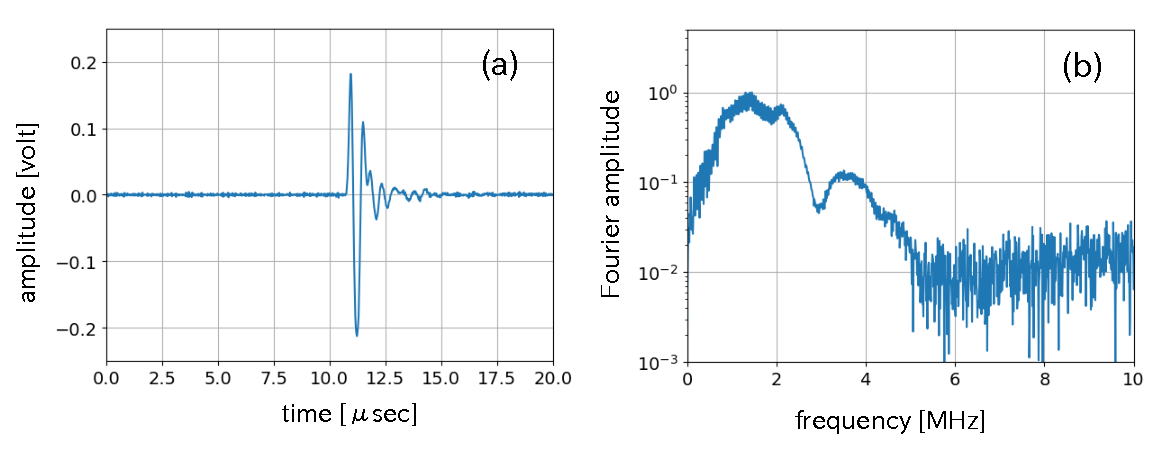
\includegraphics[width=0.9\linewidth]{Figs/fig5.eps} 
	\end{center}
	\caption{
		レーザードップラー振動計で計測した,ラインフォーカス探触子シュー先端部の振動速度波形.
	} 
	\label{fig:fig5}
\end{figure}
%--------------------
\subsection{透過波波形}
花崗岩コア供試体を用いて計測した透過波の計測結果を図\ref{fig:fig5_2}と\ref{fig:fig5_3}に示す。
これらの図には、それぞれ、入射方向の異なる6つの走時プロットが示されている。
各々の走時プロットの横軸は時間$t$($\mu$sec)を、縦軸は計測位置の$y$座標(mm)を表し,
$(t,y)$で観測された波形の振幅をカラー表示したものである。
なお、波形振幅は、最大値で無次元化している。
いずれの入射方向でも、19$\mu$sec前後に大きな振幅を持つ位相の揃った表面波が到達し、その後、
多重散乱に起因するコーダ波が、少なくとも20$\mu$sec程度継続して観測されている。
位相の揃った初動成分の振幅は場所によって大きな変動があり、波形も位置や入射方向によって異なることが分かる。
このことから、個々の観測波形のピーク位置や到達時間から、伝播速度を正確に求めることは困難と言える。
そこで以下では、群遅延から求めた群速度と、
相互相関関数によって評価した遅延時間から求めた音速を用いて、
供試体の音響異方性について調べる。
なお、
%--------------------
\begin{figure}[h]
	\begin{center}
	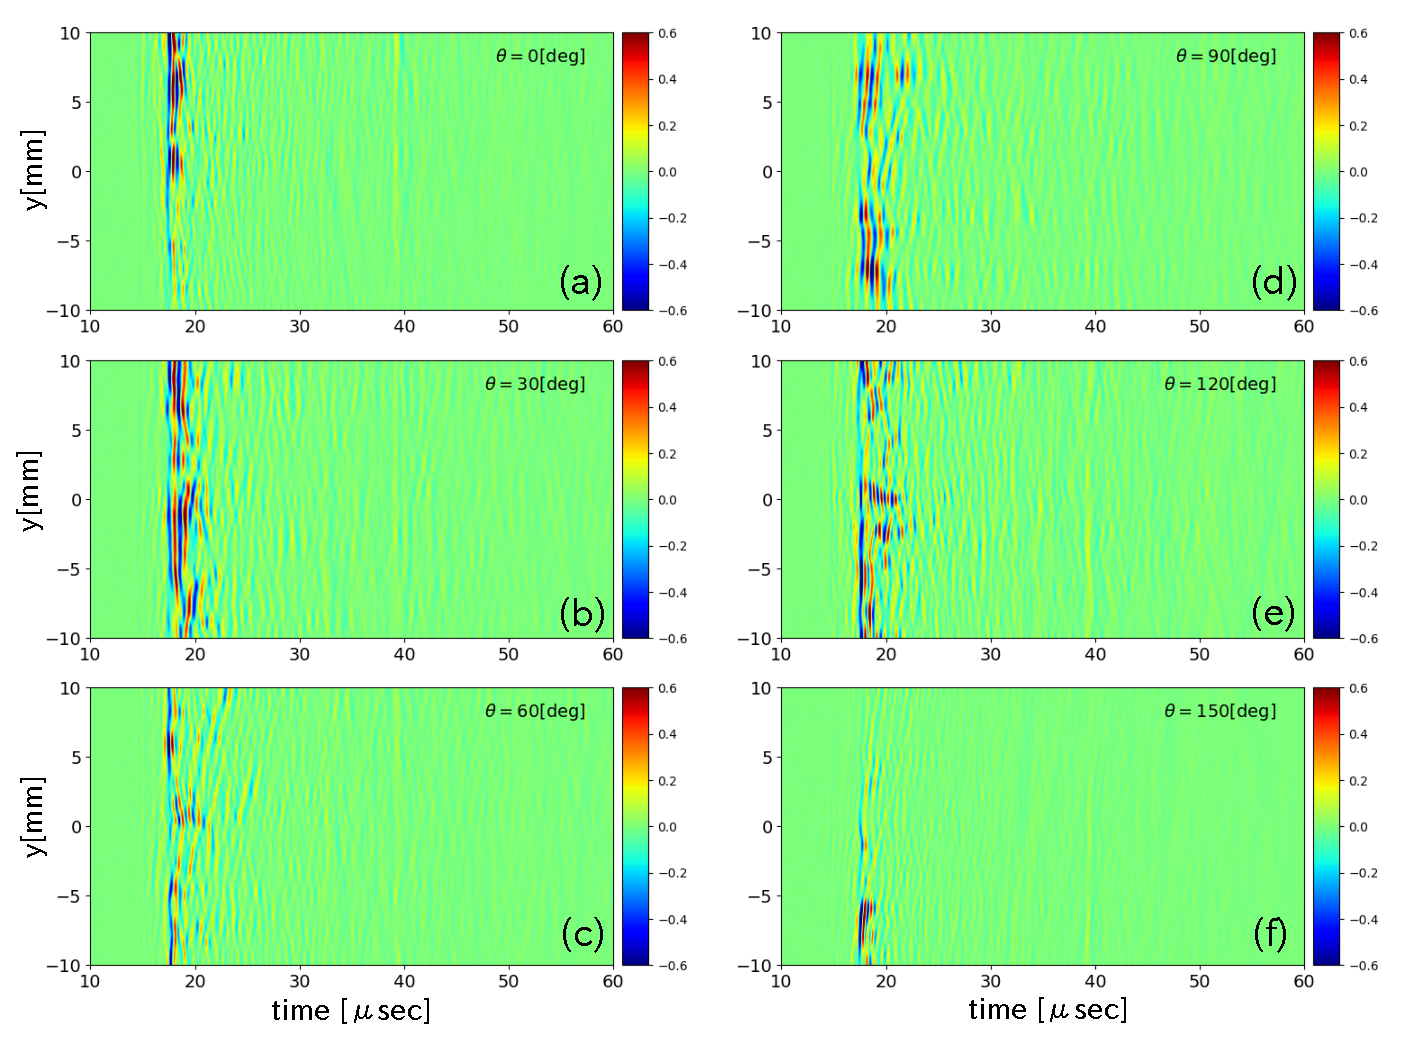
\includegraphics[width=1.0\linewidth]{Figs/fig5_2.eps} 
	\end{center}
	\caption{
		透過波波形の走時プロット(入射方向$\theta=0\sim 150^{\circ}$)
	} 
	\label{fig:fig5_2}
\end{figure}
%--------------------
\begin{figure}[h]
	\begin{center}
	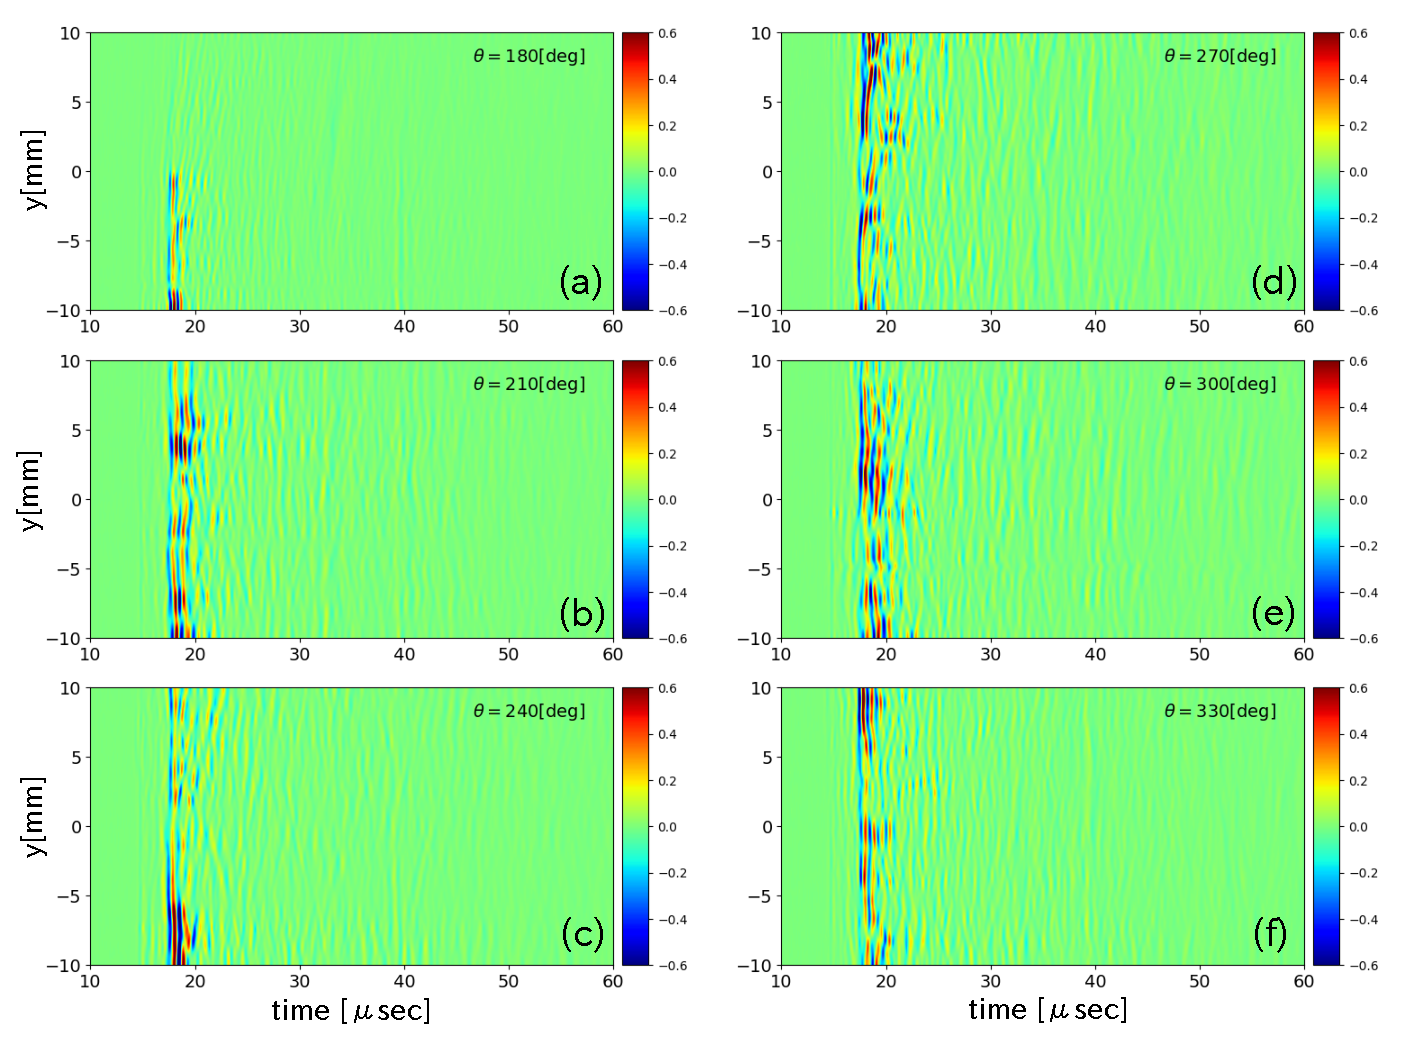
\includegraphics[width=1.0\linewidth]{Figs/fig5_3.eps} 
	\end{center}
	\caption{
		透過波波形の走時プロット(入射方向$\theta=180\sim 330^{\circ}$)
	} 
	\label{fig:fig5_3}
\end{figure}
%%%%%%%%%%%%%%%%%%%%%%%%%%%%%%%%%%%%%%%%%%%%%%%%%%%%%%%%%%%%%%%%%%%%%%
%%%%%%%%%%%%%%%%%%%%%%%%%%%%%%%%%%%%%%%%%%%%%%%%%%%%%%%%%%%%%%%%%%%%%%
\subsection{伝播速度の評価}
位相の揃った初動成分を対象として伝播速度の評価を行うために、
時間軸上で計測波形に窓関数を作用させ、初動部近傍の大きな
振幅を示す波形部分を取り出す。窓関数には、次式で与えられるButterworth関数を用いる。
\begin{equation}
	W(t;t_{1/2},m)=
	\left\{
		1+\left(\frac{t}{t_{1/2}}\right)^m
	\right\}^{-1}
	\label{eqn:Butterworth}
\end{equation}
Butterworth関数は、$m$が偶数のとき$t=0$について対称である。
その場合、$t_{1/2}$は振幅が半分となる時刻を、$m$は$t\rightarrow \pm \infty$
における減衰の速さを制御するパラメーターとなる。
ここで、$\cal R$上の位置$y$で観測される時間波形$a_{raw}(y,t)$とすれば、
窓関数をかけて取り出された波形は
\begin{equation}
	a(y,t)=a_{raw}(y,t)W(t-t_b;t_{1/2},m)
\end{equation}
と表わされる。
ここで、
\[
	t_b=18.2[\mu sec], \ \ t_{1/2}=2[\mu sec], \ \ m=6
\]
として、観測波形に窓関数を作用させると、$\theta=0$[deg]の場合、
その結果は図\ref{fig:6}のようになる。
これを、図\ref{fig:fig5_2}-(a)を比べると、初動部分の波形をほとんど変化させること無く、
コーダ波が消去されていることが分かる。
次に、$a(y,t)$の時間に関するフーリエ変換を
波形$a(t)$のフーリエ変換:
\begin{equation}
	A(y, \omega)=\int a(y, t)e^{-i\omega t}dt=\left| A(\omega) \right|e^{i\phi}
	\label{eqn:def_FFT}
\end{equation}
をFFTで計算し、スペクトログラムとして表示すると、図\ref{fig:fig7}のようになる。
スペクトログラムからは、いずれの観測点位置における波形もおよそ3MHz程度までの
周波数成分が含まれており、入射波の持つ周波数成分を大きく損なうことなく、
岩石中を超音波が透過していることが示される。
なお、図\ref{fig:fig6}と
に白の実線で示した時刻は、各観測点で得られた波形が負の最大値を示す時刻を表す。
一方、図\ref{fig:fig7}中の白の実線はフーリエ振幅の最大値を与える周波数を示す。


岩石供試体中の弾性波の平均的な伝播挙動について調べるために、入射方向毎(測線毎)に
平均波形を合成する。空間変数$y$に関する平均化作用素を
\begin{equation}
	\left< \cdot \right> := 
	\frac{1}{ \left| {\cal R} \right| }\int_{\cal R}\left( \cdot \right)dy
	\label{eqn:averaging}
\end{equation}
と表すことにすれば、波形データ${\cal D}$
\begin{equation}
	{\cal D}(\theta)=\left\{ a(y,t) \left| y\in {\cal R}, \, {\cal S}(\theta)\right.\right\}
	\label{eqn:}
\end{equation}
に対する平均波形は
\begin{equation}
	\left< a\right>(t)=
	\frac{1}{\left| {\cal R}\right|}\int_{\cal R}a(y,t)dy
	\label{eqn:def_mean_wv}
\end{equation}
で計算することができる。なお$\left| {\cal R }\right|$は、測線$\cal R$の長さを表す.
図\ref{fig:fig8}に、式(\ref{eqn:def_mean_wv})に従って計算した平均波形$\left<a \right>(t)$を
$\theta=0$[deg]の場合についてオレンジの実線で示す。この図には、ラインフォーカス探触子
シュー先端部の自由振動波形$a^{ref}(t)$を参照波形として青の実線で示している。
両者の振幅値は大きく異なることから、いずれも二乗ノルムで正規化した結果である。
これらの波形の周波数スペクトルは図\ref{fig:fig9}のようであり、透過波の平均波形では
参照波形と比べ、2MHz以上の周波数成分が小さく、伝播の過程で比較的高い周波成分が
散乱によりコーダ波に転じていることが分かる。

平均的な伝播速度の評価には、群速度$c_g$と,計測波形と参照波形の相互相関関数から評価した速度を
$c_{cor}$を用いる。
後者を、相互相関速度と呼ぶことにする。各々の定義は以下のようである。
\paragraph{群速度}
波形$v(t)$のフーリエ変換を
\begin{equation}
	V(\omega)=\int v(t)e^{-i\omega t} dt = \left| V(\omega) \right|e^{i\phi(\omega)}
	\label{eqn:phase}
\end{equation}
その、アンラップされた位相角を$\phi(\omega)$とすれば、波形$v(t)$の群遅延$t_g(\omega)$は
\begin{equation}
	t_g(\omega)=-\frac{d\phi}{d\omega}
	\label{eqn:def_gdelay}
\end{equation}
で与えられる.
図\ref{fig:fig11}は,位相角$\phi(\omega)$を平均波形$\left<a\right>(t)$と参照波形$a^{ref}(t)$
について実際に計算したものである。両者とも周波数に対して直線的に変化しており
線形位相遅れでよく近似できることが分かる。そこで、式(\ref{eqn:def_gdelay})の微分を
位相角を直線で最小2乗近似したときの直線の勾配として評価する。
そのため、$t_g$は周波数依存性はなくなり、一つの波形に対して一つの群遅延が与えられることになる。
このような方法で求めた、観測波形と参照波形の群遅延をそれぞれ$t_g, t_g^{ref}$とし、
観測波の透過距離を$L$とすれば、群速度$c_g$は
\begin{equation}
	c_g=\frac{L}{t_g-t_g^{ref}}
	\label{eqn:def_cg}
\end{equation}
で与えられる.
位置$y$で得られた波形に対して計算した群速度を$c_g(y)$とすれば、その$y$に関する平均
$\left< c_g \right>$を考えることができる。また、平均波形$<a>(t)$についても群速度を
求めることができ、以下ではこれを $\bar c_g$と表す。
$\bar c_g, \left< c_g \right>$とも測線毎(入射方向毎)に求めることができるため、
入射方向への依存性を明示的に表す必要がある際には、それぞれ、$\bar c_g(\theta), \left< c_g\right>(\theta)$
と表すことにする。
\paragraph{相互相関速度}
参照波形$a^{ref}(t)$と観測波形$a(t)$の相互相関関数を
\begin{equation}
	Cor(a,a^{ref})(t)=
	\frac{
	\int a(\tau)a^{ref}(\tau-t) d\tau
	}{
		\left\| a(t)\right\|
		\left\| a^{ref}(t)\right\|
	}
	\label{eqn:def_Cor}
\end{equation}
で定義する。$Cor(a,a^{ref}(t)$のピークを与える時刻$t_{of}$を、すなわち
\begin{equation}
	t_{of}:={\rm argmax} \left\{
		-Cor(a,a^{ref})(t)
		\right\}
	\label{eqn:def_tof}
\end{equation}
を到達時刻と考えれば,透過波の伝播速度を
\begin{equation}
	c_{cor}=\frac{L}{t_{of}}
	\label{eqn:}
\end{equation}
で求めることができる。このようにして決定した速度(相互相関速度についても)その空間平均と、
平均波形に対する速度を考えることができる。それぞれ、群速度の場合と同様に
$\bar c_{cor}(\theta), \left< c_{cor}\right>(\theta)$
と書くこととする。
図\ref{fig:fig11}は、式(\ref{eqn:def_Cor})によって計算した相互相関関数を計算した結果を
示したものである。横軸は時間$t$を縦軸は波形観測位置$y$とし、観測点毎に得られる
相互相関関数をカラー表示したものである。
図中の白の実線は相互相関関数の負のピーク位置$t_{of}$を示している。
%--------------------
\begin{figure}[h]
	\begin{center}
	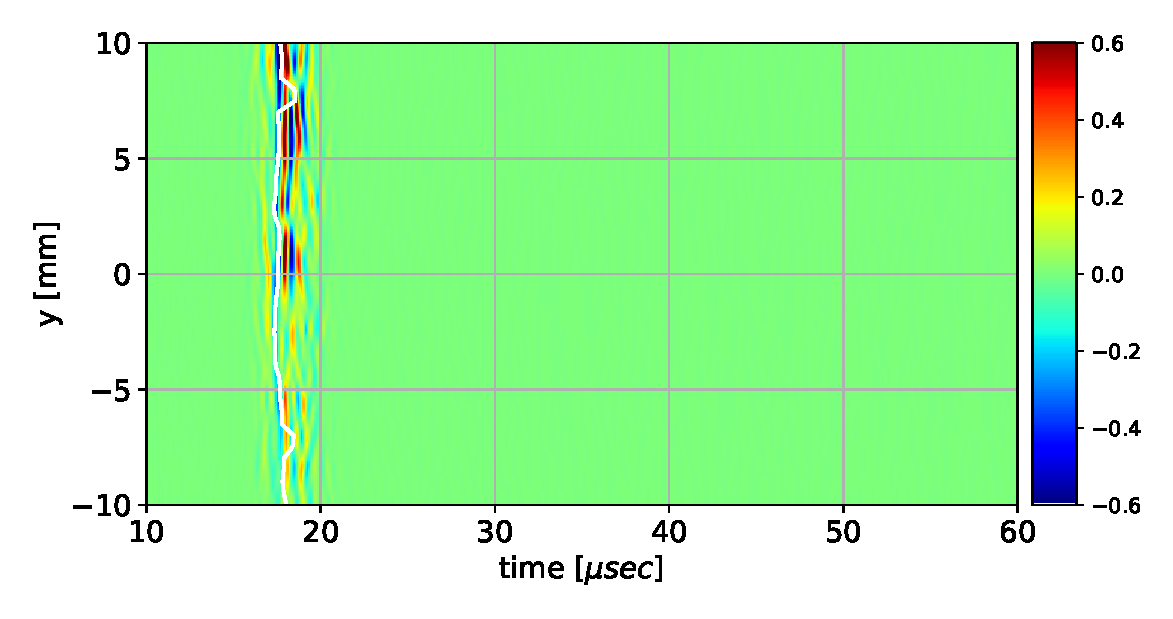
\includegraphics[width=0.7\linewidth]{Figs/fig6.eps} 
	\end{center}
	\caption{
		Butterworth窓関数で初動部分を取り出した結果の一例
		(入射方向$\theta=0^{\circ}$の場合)
	} 
	\label{fig:fig6}
\end{figure}
%--------------------
\begin{figure}[h]
	\begin{center}
	\includegraphics[width=0.7\linewidth]{Figs/fig7.eps} 
	\end{center}
	\caption{
		計測波形の初動部分に対する周波数スペクトログラム(入射方向$\theta=0^{\circ}$の場合).
	} 
	\label{fig:fig7}
\end{figure}
%--------------------
\begin{figure}[h]
	\begin{center}
	\includegraphics[width=0.6\linewidth]{Figs/fig8.eps} 
	\end{center}
	\caption{
		平均波形の時刻歴(オレンジの実線、入射方向$\theta=0^{\circ}$の場合).
		青はラインフォーカス探触子シュー先端部の自由振動波形に窓関数を
		作用させたものを参照波形として示す。
	} 
	\label{fig:fig8}
\end{figure}
%--------------------
\begin{figure}[h]
	\begin{center}
	\includegraphics[width=0.6\linewidth]{Figs/fig9.eps} 
	\end{center}
	\caption{
		平均波形(オレンジ)と参照波形(青、シュー先端部の自由振動波形)の周波数スペクトル
		(入射方向$\theta=0^{\circ}の場合$).
	} 
	\label{fig:fig9}
\end{figure}
%--------------------
\begin{figure}[h]
	\begin{center}
	\includegraphics[width=0.7\linewidth]{Figs/fig10.eps} 
	\end{center}
	\caption{
		平均波形(オレンジ)と参照波形(青)の位相スペクトル(入射方向$\theta=0^{\circ}$の場合).
	} 
	\label{fig:fig10}
\end{figure}
%--------------------
\begin{figure}[h]
	\begin{center}
	\includegraphics[width=0.7\linewidth]{Figs/fig11.eps} 
	\end{center}
	\caption{
		観測波形$a(y,t)$と参照波形$a^{ref}(t)$の時間に関する相互相関関数(入射方向$\theta=0^{\circ}$の場合).
	} 
	\label{fig:fig11}
\end{figure}
%--------------------

